\documentclass{article}

\usepackage{arxiv}

\usepackage[utf8]{inputenc} % allow utf-8 input
\usepackage[T1]{fontenc}    % use 8-bit T1 fonts
\usepackage{hyperref}       % hyperlinks
\usepackage{url}            % simple URL typesetting
\usepackage{booktabs}       % professional-quality tables
\usepackage{amsfonts}       % blackboard math symbols
\usepackage{nicefrac}       % compact symbols for 1/2, etc.
\usepackage{microtype}      % microtypography
\usepackage{lipsum}
\usepackage{graphicx}
\usepackage{physics}
\graphicspath{ {./images/} }


\title{Research Proposal for IGP(A) Program at Tokyo 
Institute of Technology}


\author{
 Shiwen An \\
 High Energy Accelerator Research Organization, KEK \\
  Tsukuba, Japan \\
  \texttt{shiwen.an@cern.ch} \\
  %% examples of more authors
  %  \And
  % Konstantinos Slavakis \\
  % Department of Information and Communication Engineering\\
  % Tokyo Institute of Technology\\
  % Yokohama, Kanagawa\\
  % \texttt{slavakis.k.aa@m.titech.ac.jp} \\
  %% \AND
  %% Coauthor \\
  %% Affiliation \\
  %% Address \\
  %% \texttt{email} \\
  %% \And
  %% Coauthor \\
  %% Affiliation \\
  %% Address \\
  %% \texttt{email} \\
  %% \And
  %% Coauthor \\
  %% Affiliation \\
  %% Address \\
  %% \texttt{email} \\
}

\begin{document}
\maketitle
\begin{abstract}
The research proposal focuses on development of 
state-of-art Quantum Computing algorithms for Machine Learning 
and Signal Processing. The more detailed 
studies lie in field of Quantum Machine Learning algorithms, with combination 
of data analysis techniques in Riemannian Manifolds. Meanwhile, the research 
expects to expand the application of Quantum Fourier Transform in signal 
processing field. The encoding in quantum computing will also be 
included as supplementary study. 
\end{abstract}

% keywords can be removed
\keywords{ 
  Quantum Signal Processing \and Quantum Fourier Transform \and 
  Quantum Machine Learning \and Variational Quantum Circuit \and 
  Variational Shadow Quantum Learning \and Quantum Kernel Method \and 
  Quantum Block Encoding }

*The citation is not precisely managed. 

\section{Your research topic in Japan:
Describe articulately the research you wish
to carry out in Japan.}
\textbf{Research theme:} Quantum Computing Algorithms for 
Machine Learning and Signal Processing.  \newline 
\newline
Quantum Computing was postulated in the early 1980s as way to 
perform computations that would not be tractable with a classical 
computer. Currently, at Noisy Intermediate-Scale Quantum (NISQ)
era, 50 to hundreds of qubits are available for algorithm designs \cite{aps_review}.
So far, companies like D-wave implemented quantum computers specialized 
quantum annealing and Xanadu implemented Photonic Quantum Computers with 
216 qubits available. 
Many quantum algorithms have already been  
developed with the aim at exploiting the capacity of the 
hardware for machine learning and signal processing application. 
An interesting question is whether there are efficient 
quantum machine learning algorithms could approach or outperform the 
existing machine learning algorithms. 
The Variational Quantum Circuits (VQC) are demonstrated to 
approximate the Deep Reinforcement Learning for decision-making 
and policy-selection \cite{ieee_vqc}. 
Within decades of research, a universal fault-tolerant 
quantum computer that can solve efficiently problems such 
as integer factorization and unstructured database search using 
millions of qubits are expected to be developed \cite{qml_hep}. 

\textbf{Notations: } \newline 1. Hilbert space: in quantum mechanics, 
the state of a physical system is represented by a vector in 
a \textit{Hilbert space}: a complex vector space with an inner product. \newline
2. \textit{Dirac notation} is used to represent the vectors in the 
Hilbert space, denoted by $\ket{v}$, called ket, where $v$ is 
some symbol which identifies the vector. One could equally well 
use something like $\overrightarrow{v}$ or $\text{\textbf{v}}$. A 
multiple of a vector by a complex number $c$ is written as 
$c\ket{v}$ $\implies$ think of it as analogous to $c \overrightarrow{v}$ 
or $c \text{\textbf{v}}$. \newline 3. In Dirac notation the inner 
product of the vectors $\ket{v}$ with $\ket{w}$ is written as $\braket{v}{w}$. 
This resembles the ordinary dot product $\overrightarrow{v} \cdot \overrightarrow{w}$, 
thus think of $\overrightarrow{v}^{*} \cdot \overrightarrow{w}$.

\subsection{Prior Literature and Current Development on Quantum Computing Algorithms}

\textbf{Quantum Machine Learning} Machine learning has been used in various fields for a long time, 
with algorithms like deep neural network (DNN), binary decision tree (BDT),
convolutional neural network (CNN), Generative adversarial network (GAN) and 
etc. Recent years, 
the robust development of quantum computing has also brought people 
VQC, Quantum Kernel Methods, Variational Shadow Quantum Learning (VSQL), and Quantum Generative 
Adversarial Network (Quantum-GAN). These new approaches solve 
the clustering, classification, discrimination problems in 
Quantum Computing. Most of them take advantages of exponential 
improvement in computational speed of quantum computer and are expected 
to have better performance than its classical version of algorithms. 

\begin{figure}[h]
  \begin{center}
    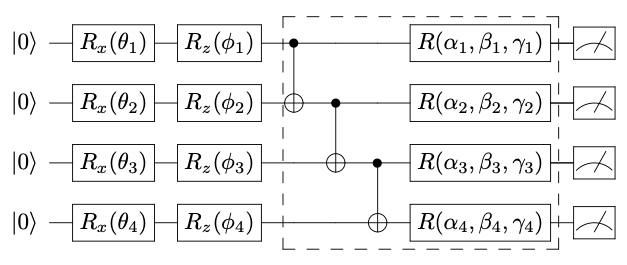
\includegraphics[width=0.58\textwidth]{vqc.png} 
    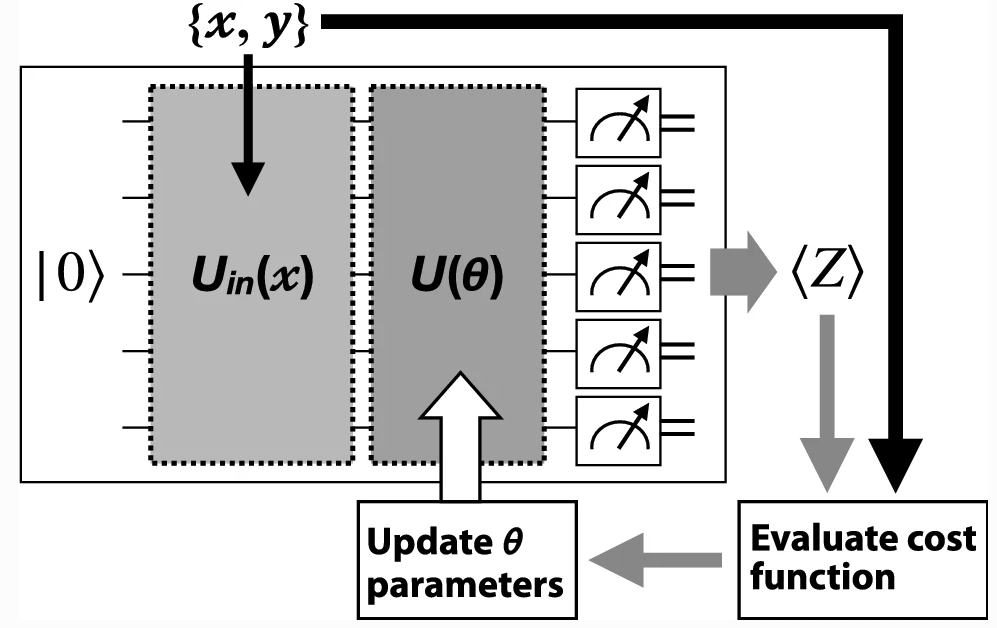
\includegraphics[width=0.38\textwidth]{vqc1.png} 
  \end{center}
  \caption{The generic variational quantum circuit 
  architecture and procedure for optimization. The 
  inputs go through encoding, the unitary matrices, 
  measurement, lost function evalution and then 
  update parameters.}
\end{figure}

\textbf{Quantum Signal Processing}
The Fourier transform occurs in many different classical computing 
fields, especially signal processing. The decompose of wave from 
silicon detectors, image processing from CMOS detector, the noise filtering
and more all require use of Fourier Transform. The quantum Fourier 
transform is the quantum implementation of the discrete Fourier 
transform over the amplitudes of a wavefunction. It is part of 
many quantum algorithms, most notably Shor's factoring algorithm
and quantum phase estimation. 

Borrowed from Qiskit's notation, the classical discrete Fourier Transforms
act on vector $x = (x_0, x_1,...,x_n)$ and its mapping to vector $y = (y_0, y_1,...,y_n)$
according to formula:
\begin{equation}
  y_k = \frac{1}{\sqrt{N}} \sum^{N-1}_{j=0} x_j \omega_N^{jk}
\end{equation}
Where $\omega_N^{jk} = e^{2\pi i \frac{jk}{N}}$. The quantum state
$ \ket{X} = \sum^{N-1}_{j=0} x_j \ket{j} $ and mapped to $ \ket{Y} = \sum^{N-1}_{k=0} y_k \ket{k} $
and the map could therefore be expressed as:
\begin{equation}
  \ket{j}  = \frac{1}{\sqrt{N}} \sum^{N-1}_{j=0} \omega_N^{jk} \ket{k}
\end{equation}
Or the unitary matrix:
\begin{equation}
  U_{QFT}= \frac{1}{\sqrt{N}} \sum^{N-1}_{j=0} \sum^{N-1}_{k=0}  \omega_N^{jk} \ket{k} \bra{j}
\end{equation}
There are already well published paper and books for quantum Fourier transform \cite{qc_book}.

\begin{figure}[h]
  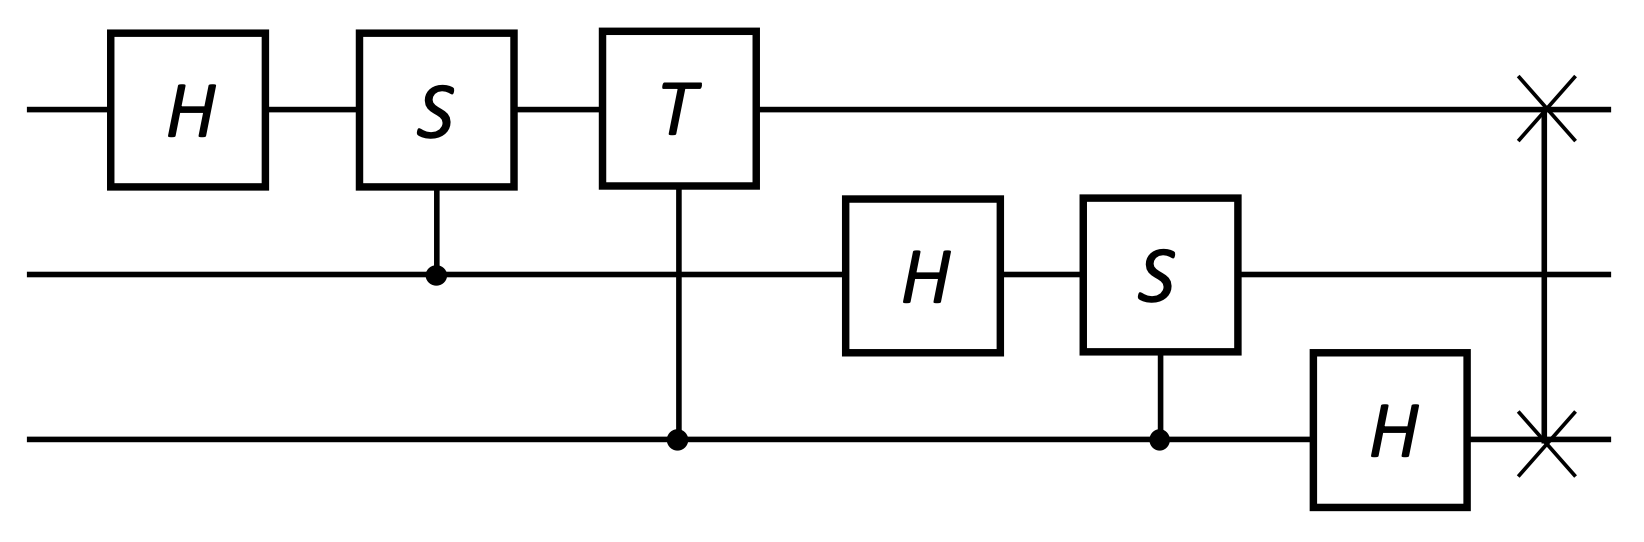
\includegraphics[width=0.48\textwidth]{qft2.png}
  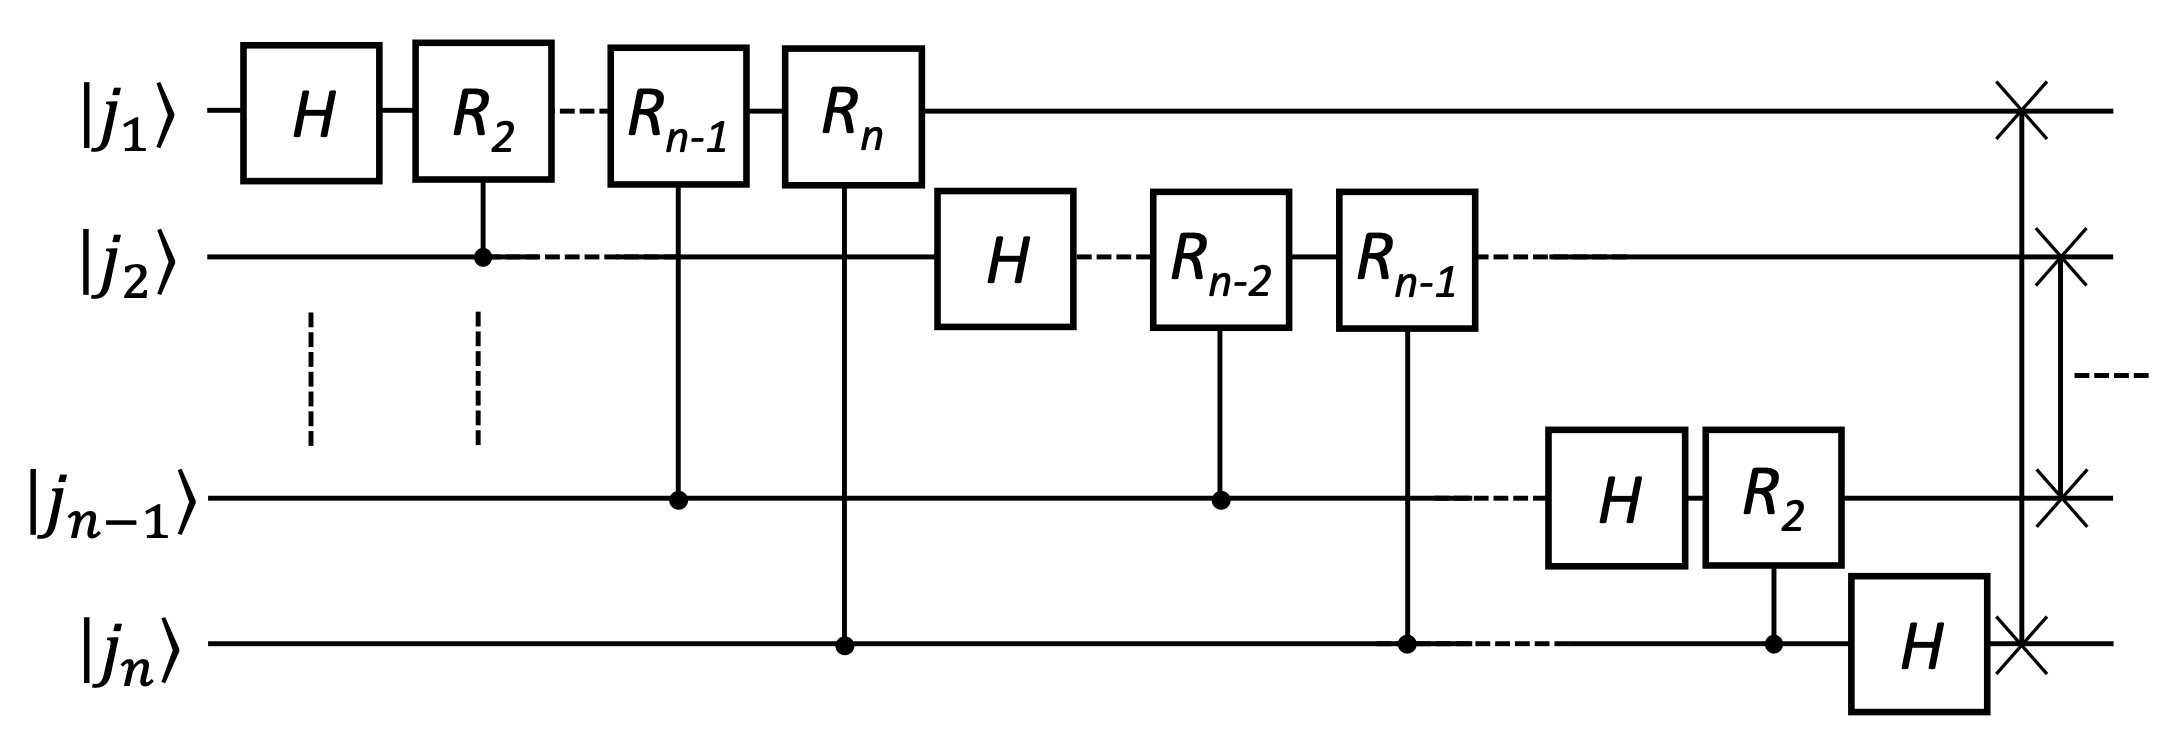
\includegraphics[width=0.48\textwidth]{qft1.png}
  \caption{The quantum Fourier Transform Circuit for 3 qubits only and 
  n different qubits}
\end{figure}

 
\subsection{Motivation for working on Quantum Machine Learning and Quantum Signal Processing}

\textbf{Quantum Machine Learning:}  Before the robust 
development of machine learning, people question about 
what to do with machine learning. Now it turns similar 
question to quantum machine learning. What is the advantages of 
quantum version of machine learning over the classical 
machine learnign? What is the benefit if one just translate
the classical algorithm? If current quantum algorithms could 
solve some problems, is there any quantum algorithm that have 
better performance?
One interesting answer is to 
combine quantum machine learning algorithms with clustering 
algorithms using Riemannian Manifold, and benefit from 
advantages in both algorithms. In Riemannian Manifold, 
reproducing Kernel Hilbert space(RKHS)
plays important role in extracting the 
features. Also in quantum kernel method, RKHS is also 
form before input to the quantum circuit for further learning, 
with additional encoding required for quantum circuit processing. 
The shared procedure provides idea to improve the existing 
algorithms using Riemannian Manifold and combine it to 
quantum kernel method, either deriving the completely new algorithm or 
improving the existing clustering algorithms would be interesting. 
\cite{qml_kernel} \cite{qml_ibm} \cite{qml_ibm2}

\textbf{Quantum Signal Processing:} 
Moreover, with quantum Fourier transform, could we benefit from 
formation of Hilbert space in quantum computer and bring it to 
signal processing field and more? Could we actually prove the 
universal advantages of quantum computing algorithms over the 
classical algorithms in machine learning and signal processing? 

1. \textbf{QFT ready Original Signal State } One important question is:
\textit{
Can we use the quantum Fourier transform to speed up the 
computation of the Fast Fourier Transform or Discrete Fourier Transform?} 
In Issac Chuang's book, he considered the amplitude in a quantum 
computer cannot be directly accessed by measurement. Moreover, Chuang 
thinks there is no way of determining the Fourier transformed 
amplitudes of the original states. However, in image processing field, 
different Quantum Image Representation were proposed and some quantum analog 
representation of classical images is demonstrated. Such progress in recent 
year motivates me to rethink about the possible application of QFT in 
signal processing.   \newline

2. \textbf{Efficiency Improvement} The Shor's algorithm is a 
quantum computer algorithm for finding the prime factors of an integer. 
Shor's algorithm runs polynomial time and allows us to find prime decomposition of very big 
numbers in $O ((log N)^3)$. One of the important factors such algorithm is so efficient is 
due to the efficiency of quantum Fourier transform. The discrete Fourier transform on 
$2^n$ amplitudes can be implemented as quantum circuit consisting of only $O(n^2)$ Hadamard gates
and controlled phase shift gates using n qubits. Compared with discrete Fourier transform, 
which takes $O(n 2^n )$ bits in classical computer. \underline{Such exponentially improvement 
efficiency using quantum Fourier transform}, motivates me to think how to apply this 
to imaging processing, noise filtering and more. With more detailed study on 
classical algorithms in signal processing, the exploration of quantum 
Fourier transforms and formation of quantum signal processing framework based on 
this idea would be really interesting. 

\section{Study program in Japan:
(Describe in detail and with specifics - particularly
concerning the ultimate goal(s) of your research in Japan)
}

\subsection{Research Objectives}
The ultimate target is to develop breakthrough algorithms
 in quantum machine learning and quantum signal processing. 
 Developing quantum machine learning algorithms, I hope to 
find the one outperforms current classical machine learning 
algorithms. Moreover, in quantum signal processing part, I expect to 
develop algorithms to complete tasks considered not possible in 
the past. 
\textbf{
\renewcommand{\labelenumi}{\Alph{enumi}}
\begin{enumerate}
  \item Quantum Machine Learning: Quantum Machine Learning 
  \item Quantum Signal Processing: Quantum Fourier Transform
  % \item Quantum Signal Processing: Encoding Theory 
\end{enumerate}
}
A. The existing Kernel or Reproducing Kernel Hilbert space in 
the Riemann Manifold Method will be enhanced or improved 
models for data analysis using Quantum Kernel Method. Combination of these two algorithms
could possibly solve the clustering problems in Riemannian Manifold 
and improve the time and space exponentially. 

B. In imaging analysis, Fourier transform is definitely an unavoidable technique. 
In analog signal processing, we could apply the quantum Fourier transform and 
the classical discrete Fourier transform. Then compare their differences and how
quantum Fourier transform could possibly enhance the classical result to get started.
Later, several goals for working on Quantum Fourier Transform:
\begin{enumerate}
  \item Forming algorithms could possibly enhance or replace the classical
  discrete Fourier transform. Such replacement may improve classical
  algorithms to achieve better performance in feature extraction, like noise filtering, 
  image processing and etc.
  \item By the theory of Big-O, the quantum Fourier transform is exponentially
  faster than classical discrete Fourier transform. Verification the efficiency 
  improvement would also be a nice work to implement and get started. 
\end{enumerate}

% C. Encoding is essential for quantum computing. Before precossing data 
% into the variational quantum circuit, or any type of quantum circuit, 
% encoding of data using angle encoding or amplitude encoding are mandatory. 
% The efficient encoding algorithm is considered as side product of research 
% in quantum machine learning and the quantum signal processing. 

\subsection{Reseaerch Method}
With motivation in last section, the method to achieve 
research objective A B C will be explained in more details. 

\textbf{Quantum Kernel Method} Among all the 
Quantum Machine learning algorithms, Quantum Kernel 
Method plays an important role for classification problem using 
large dimension of quantum Hilbert space. Traditionally, 
kernel methods for machine learning 
are ubiquitous for pattern recognition, 
with support vector machines (SVMs) being the most well-known method 
for classification problems. 
In kernel methods, the access to the feature space is facilitated 
through kernels or inner products of feature vectors. 
In quantum computing, access to the Hilbert space of quantum states
 is given by measurements, which can also be expressed 
 by inner products of quantum states. \cite{qml_kernel2}

There are limitations to the successful 
solution to such problems when the feature space becomes large, 
and the kernel functions become computationally expensive to estimate. 
Then, people start to think of computational speed-ups afforded by 
quantum algorithms. The exploitation of an exponentially 
large quantum state space through controllable 
entanglement and interference could resolve current limitations. 

\textbf{Clustering Problems in Riemannian Manifolds}
Currently in Machine Learning and Signal Processing field, 
people study the learning from data/features which 
Numerous well-known features in signal processing 
and machine learning belong to Riemannian manifolds, like 
correlation matrices, orthogonal matrices, fixed rank linear 
subspaces and etc. 

Many learning tasks could be studied with forming feature 
space and Riemannian Manifold. The state clustering, 
connectivity among network nodes that stays fixed over a 
time interval. The community detection, subgroup detection 
of nodes within a single state/layer. Subnetwork-sequence 
clustering, sequence of subgroups of nodes with changing state. 
The algorithms study benefits understanding of the brain networks 
and its relation with Alzheimer disease, autism, depression and more.

\textbf{Quantum Machine Learning: Quantum Kernel Method and its
application on Riemannian Manifold}
\begin{figure}[h]
  \begin{center}
    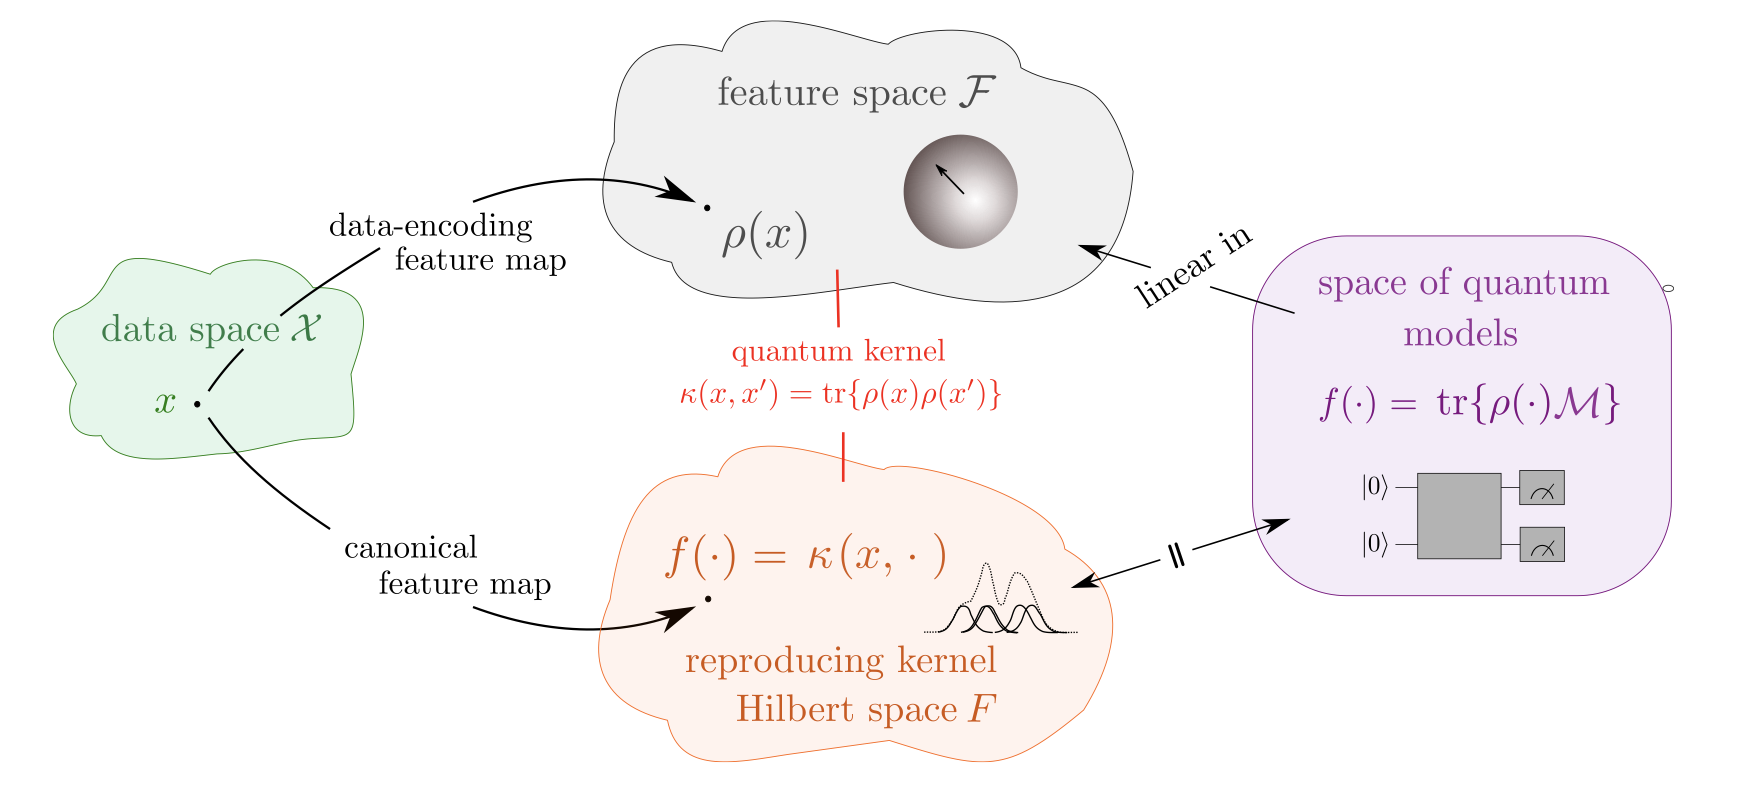
\includegraphics[width=0.35\textwidth]{kernel1.png}
    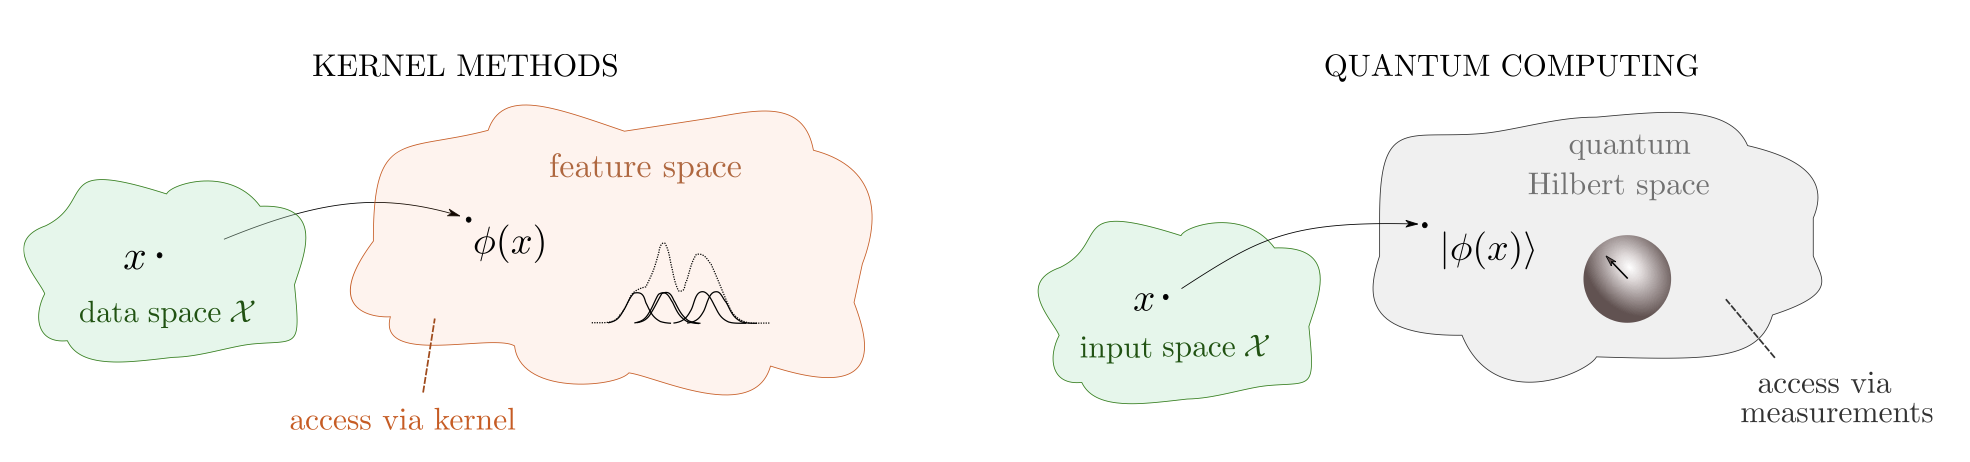
\includegraphics[width=0.63\textwidth]{kernel2.png}    
  \end{center}
  \caption{Overview of the link between quantum models 
  and kernel methods.}
\end{figure}
In practice, the feature space's demensionality 
sometimes can be extremely large. While not 
tackling these feature vectors directly, we 
implicitly analyze the feature vectors by 
only accessing their inner products in the 
feature space, which gives the classical kernel functions K(,):
\begin{equation}
  K(x_i, x_j) = \phi(x_j)^T \phi(x_i)
\end{equation}
With support vector machine (SVM), a given dataset 
$T = \{ (x_1, y_1), ..., (x_m, y_m)\}$ in $Z_2$, and 
a hyperplane $(w,b)$, a SVM can assign labels through
signs of the decision function, as:
\begin{equation}
  y_{\text{pred}} = \text{sign} ( <w,x> +b)
\end{equation}
Also, separation by mapping them into a feature space
is another solution, where $y_{pred} = sign( <w', \phi(x)> +b')$ and 
$w' = \sum_i \alpha_i \phi(x_i)$. with Lagrangian multipliers 
$\alpha_i$. Then, under constraints $\alpha_i \leq 0 $ and 
$\sum_i y_i \alpha_i = 0$, we can compute the optimal 
$\alpha_i^{*}$, thus the optimal hyperplane by maximizing: 
\begin{equation}
  \sum_i \alpha_i - \frac{1}{2} \sum_{i, j} \alpha_i \alpha_j y_i y_j 
  \phi(x_j)^T \phi(x_i)
\end{equation}
From the equation above, we only need the inner product of feature 
vectors $\phi(x_j)^T \phi(x_i) = K(x_i, x_j)$, which is the above 
mentioned kernel function. With such idea, $y_{\text{pred}}$ is: 
\begin{equation}
  y_{ \text{pred}} = \text{sign} ( \sum_i \alpha_i^* K(x,x') +b')
\end{equation}
With the idea of classical methods, the essentials of 
quantum kernel methods are the same, if we map a 
classical data vector x into quantum state $\ket{\phi(x)}$
by encoding circuit $U(x)$ as follows:
\begin{equation}
  U(x) \ket{0^{N}} = \ket{\phi(x)}
\end{equation}
The quantum kernel function is the inner products of 
two quantum feature vectors in the Hilbert space:
\begin{equation}
  K^Q_{ij} = |\bra{\phi(x_j)} \ket{\phi(x_i) }|^2 = |\bra{0^{\bigotimes N}} U^{\dagger}(x_j) U(x_i) \ket{ 0^{\bigotimes N }} |^2
\end{equation}
This kind of kernel manipulation could then feed into 
the common variational quantum circuit learning method 
and then go through the training as the circuit below. 
\begin{figure}[h]
  \begin{center}
    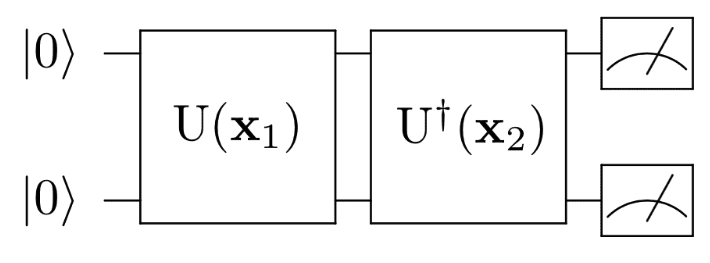
\includegraphics[width=0.55\textwidth]{kernel.png}    
  \end{center}
  \caption{Simple demo for quantum circuit in kernel method}
\end{figure}
One consideration is the number of 
qubit and the Hilbert space's dimensionality. 
The Hilbert space's dimensionality grows exponentially 
with the number of qubits, nearly all quantum states
will be perpendicular to each other when we have a large 
number of qubits. The kernel matrix will converge 
to identity matrix $K_{ij} = K(x_j,x_i) ~ I$, 
and the kernel methods fail. One solution here is 
to extract the "features" from Hilbert space and 
then construct the kernel function with 
these extracted features. The projected quantum 
kernel is therefore proposed: 
\begin{equation}
  K^P (x_i,x_j) = exp(-\gamma \sum_k \sum_{p \in M} 
  (Tr(P \rho(x_i)_k)-Tr(P \rho(x_j)_k))^2)
\end{equation}
where $\rho(x_i)_k$ the reduce density matrix of 
qubits $k$ , $M$ a set of measurements on 
the reduce density matrix. Then, the idea for combination of 
the Quantum Kernel Method in RKHS with the
Fast Sequential Clustering in Riemannian Manifolds will be 
illustrated.

\textbf{Combine with Clustering Problem on Riemannian Manifold}

In paper Fast Sequential Clustering in Riemannian
manifolds for Dynamic and Time-series-Annotated Multilayer Networks. This
work focus on building a sequential-clustering framework able to address
a wide variety of clustering tasks in dynamic multilayer (brain) networks
via the information extracted from their nodal time-series.
I consider two essential algorithms are here:
\begin{enumerate}
  \item feature extraction from time-series
  \item Riemannian Manifolds
\end{enumerate}
This work claims that the rich geometry of 
(not necessarily embedded in Euclidean spaces) Riemannian manifolds 
allows latent feature patterns to unfold to the benefit of all of 
the aforementioned network-clustering tasks.

The Grassmanian $Gr(\rho, M)$ is defined as the collection 
of all linear subspaces fo $R^M$ with rank equal to $\rho$. 
Motivated by the success of kernel methods in capturing 
non-linearities in data, user could define RKHS $H$ with its associated
reproducing kernel function $\kappa(*,*)$ and the mapping 
could extract features from the Grassmanian $Gr(\rho, M)$. In such 
algorithm, Kernel correlations 
$K_v^{(l)}[t] = \phi_v^{(l)} \bigotimes_H \phi_v^{(l)}$ itself 
as a feature in Riemannian manifold of $P(S)D(T_w)$ of 
positive-(semi)definite matrices, of dimension $T_W (T_W+1)/2$,
to take advantages of the rich Riemannian Geometry of $P(S)D(T_w)$

With proper study of the quantum kernel method, the kernel relation 
here could be possibly replace with $
  K^P (x_i,x_j) = exp(-\gamma \sum_k \sum_{p \in M} 
  (Tr(P \rho(x_i)_k)-Tr(P \rho(x_j)_k))^2)
$
then process through the quantum computer. Based on processing 
result through quantum kernel method, the features could be well 
discovered through time interval or more. It could expect that in 
the future, applications facing large-scale networks and data, e.g., very long 
nodal time-series, if the quantum kernel method is computationally efficient clustering 
framework.  Quantum kernel method could operates together 
on data and features 
and carries through all of the network clustering tasks in 
Riemannian manifolds. 

\textbf{Quantum Signal Processing: Quantum Fourier Transform and Image Processing}\newline
The structure for the development of Quantum Signal Processing starts from
measurement. The wave break down by using Fourier transform's quantum analog
part, Quantum Fourier Transform (QFT). The Quantum Fourier transform could
particularlly decompose into a product of simpler unitary matrices.
With Simple decomposition, the discrete Fourier transform on $2^n$ amplitudes
can be implemented as a quantum circuit consisting of $O(n^2)$ Hadamard
gates and controlled phase shift gates. 


\textbf{Image Processing:} The quantum-analog representation of classical images, the pixel value 
of $i^{th}$ row and the $j^{th}$ column can be stored as:
$\ket{pixel_{i,j}} = \cos(\frac{\theta_{i,j}}{2}) \ket{0} + 
\sin (\frac{\theta_{i,j}}{2}) \ket{1}$ as formed in \textbf{Qubit Lattice} model.
Other image representations like \textbf{Flexible Representation of 
Quantum Images} (FRQI) exists: 
\begin{equation}
  \ket{I(\theta)} = \frac{1}{2^n} \sum_{i=0}^{2n-1} (sin(\theta_i) \ket{0} + cos(\theta_i)\ket{1}) \ket{i}
\end{equation}
it actually maps each pixel's grayscale value to the amplitude as well as 
captures the corresponding positions in an image and integrate them into 
a quantum state. Where $\theta$ encodes pixel value of the corresponding 
position $\ket{i}$. The FRQI representation maintains a normalized state 
and the representation space decreases exponentially compared to the 
classical image due to the quantum states' superposition effect. 
Moreover, image representation like \textbf{Novel Enhanced Quantum Representation} (NEQR) exists:
\begin{equation}
  \ket{I} = \frac{1}{2^n} \sum^{2^{2n} -1 }_{y=0} \sum^{2^{2n} -1 }_{x=0} \ket{f(y,x)} \ket{y x}
\end{equation}
Such method uses the basis state of a qubit sequence to 
store the grayscale value of every pixel instead of 
probability amplitude encoded in a qubit in FRQI. 
These representations for images provide possible application on 
quantum Fourier transform. There are already some study using quantum kernel 
method to work on classification. If properly organized, edge detection, filtering 
and more could be realized in thoroughly different method from today. The 
data for testing the new algorithm could use public dataset like 
\textbf{MNIST} dataset or \textbf{CIFAR-10} dataset. If the 
overall new algorithm works with exceptional performance, the 
dataset with fMRI could be used. 

More importantly, the Quntum Convolutional Neural Network (QCNN) exists for 
classification and image processing \cite{qml_cnn}. Parameterized 
QCNN was benchmarked for classical data classification with 
high accuracy and the best case being about 99\% for MNIST and 
about 94\% for Fashion MNIST \cite{qml_cnn1} \cite{qml_cnn2}. 
With combination of QCNN, quantum Fourier Transform, and Quantum 
Representation of Images. Setup of Quantum Fourier Convolutional Neural Network (Q-FCNN)
is possible. The big picture for such algorithm is:
\begin{enumerate}
  \item Classical Image Data Encoding to Quantum Image Representation
  \begin{enumerate}
    \item build up kernels for images then convert each kernel to Quantum Representation
    \item Directly take input images to Quantum Representation
  \end{enumerate}
  \item Using Quantum Fourier Transform take Image Representaions to Fourier Space
  \item MERA QCNN take QFT transfered data
  \item Inverse Quantum Fourier Transform
\end{enumerate}

Here is just one possibility for new quantum algorithm in field of signal processing. Other
simpler models using previously mentioned VQC is also an option. 

\subsection{Tentative Plan/Timetable}
The first two years are filled with more details 
and later three years would be planned at later stage. 

\begin{center}
  \begin{tabular}{c|c|c}
    Year & Content & Outcome \\
    \hline
    2023 - 2024 &  Signal Processing and Differential Geometry Theory Courses& Learn basics \\
                &  Seminars on Quantum Machine Learning &  work with Labmates \\
                &  Simple Research on Application Oriented Studies & Local Conference Talks \\ 
    2024 - 2025 &  Algebraic Geometry and Quantum Computing Theory Courses & Learn basics \\
                &  Seminars on QML and Quantum Signal Processing  & work with Labmates \\
                &  Summarize First two years of study & Journal/Conf Publication \\
                & & Master Thesis \\
    \hline
    2025 - 2026 &  Research on Quantum Fourier Transform  & Journal/Conf Publication\\
    2026 - 2027 &  Research on QFT and Related Encoding Theory  & Journal/Conf Publication \\
    & Research on Quantum Image Processing & International Conference Talks \\
    2027 - 2028 &  Summarize Five years of study & PhD Thesis and Graduation 
  \end{tabular}
\end{center}


\textbf{Research Originality:}
Quantum computing and quantum information science became a hot topics in 
recent years. \cite{qml_hep}
Once there is breakthrough on Noise intermediate Scale quantum era NISQ. All 
the research could take the data analysis, machine learning, signal processing 
to next level. As Tokyo Insitute of Technology has quite strong bond with 
IBM and development of quantum computer, I expect the new methods I provide 
would not only run on the emulators on super computer, but also on latest real 
quantum computers.

Moreover, with connection globally, not only using the fMRI data in brain locally 
at Tokyo Institute of Technology, collaboration with people from international 
institute like MIT, University of Chicago, University of Hong Kong, CERN, KEK and 
more are all possible. The clustering algorithms anti-kt is already the 
default on clustering analysis for jets in colliders and there are so 
many possibilities my research could create a new methodology for 
all types of study in natural science and broader human society. 


\section{Present Field of Study}

The pixel hit information plays vital rule for the charge particle track reconstructions,
especially for flavor tagging such as c-, b-quark jets or hadronic tau identifications, where
they form as a colimated spray of the charged particles. The track reconstruction software
has been developed to identify such particles in the dense environment of the very narrow
space using the neural network technique. Meanwhile, the pixel detector has been experienced
significant radiation damage that degradates the performance. The pixel hits will be lost at
most 50\% of efficiency in b-layer in the end of RUN3, in turn lost the performance for the
cluster classification to split or merge the associated cluster in the dense track reconstruction.
The evaluation of the radiation damage of the pixel detector and modeling of the pixel cluster
classification in the simulation is thus critical to improve the systematic uncertainties through
RUN3.
The task devotes to monitor the pixel cluster classification performance using the
$Z \rightarrow \tau \tau$ events. The hadronic tau with 3-prong decay mode is a clean source for the dense
tracking. The task first constructs clean dataset of the $Z \rightarrow \tau \tau$ with 3-prong final state, then
the pixel clustering is compared with the simulation in a various view in term of the radiation
damage. The produced dataset would be useful for many area for the tracking aspect as further
optimization of the neural network training.


% \section{Present Field of Study}

% During my undergraduate period, my field of study was Atomic, 
% Molecular and Optical physics. More specifically in optical 
% science, I was exploring the High Harmonic Generation property
%  of various light sources. Instead of commonly seen 2nd and 
%  3rd order harmonic generation for the laser light, the lab
% I worked for is trying to generate light with higher harmonics
% like 30th order, or even higher 4000th order harmonics. 
% In the beginning, the research starts with simulation codes
% (with Matlab) of tunnel ionization to find potential of the
%  perturbed system. Meanwhile, I studied and utilized software
%   engineering techniques (with C\#), some basic circuit 
%   construction and computer vision knowledge to make 
%   a 3D machining station with a femtosecond laser. 
%   The machining station is used for precise fabrication 
%   under micrometers. These tools empower the entire lab 
%   experiment and help with further development. 
% Another field of study I spent my time heavily on is 
% the Condensed Matter Physics. After finishing courses 
% in electrodynamics and quantum mechanics, I chose several 
% courses in experimental and theoretical condensed matter physics.
%  For the experimental course, we formed a team of three and 
%  completed research in 10 weeks specialized in analysis of 
%  YBCO superconductors with Raman spectroscopy. For the 
%  theoretical course,  Landau Level, various techniques in 
%  quantum information and some other state-of-art models in 
%  condensed matter physics. All the studies here are trying 
%  to understand the complexity in fundamental physics. 
%  In general, these two fields of studies help me prepare 
%  for hands-on experience in experimental physics and 
%  enough intuition to understand the model proposed in 
%  theoretical physics.

% However, after shifting the field of study after 
% I came to Japan, there are plenty of changes in my 
% field of Study. I started working on the ATLAS 
% experiment and its silicon pixel detector upgrade
%  for High Luminosity LHC. Quite frequently, 
%  we have to consider the detector’s signal from 
%  the fundamental level. Like the photon collides 
%  with the detector, generates electron hole pair 
%  in the semiconductor and data analysis. Here I 
%  improve the high level trigger efficiency of HH to bbtautau 
%  analysis using the Monte Carlo data sample.
 
% Moreover, based on existing data, I start to 
% apply many quantum machine learning algorithms 
% to the Higgs particle signal analysis. Collaborate 
% with researchers from Chicago and Hong Kong, 
% I applied the Variational Quantum Circuit Algorithms[], 
% Variational Shadow Quantum Learning Algorithms[VSQL] and 
% Quantum Kernel Methods to the data obtained from LHC. 
% The experience working on the field of data analysis 
% and some signal processing field makes me interested 
% in working on the more engineering oriented studies.
%  and hopefully I could develop some useful algorithms 
%  or method which could improve the existing signal 
%  processing field. Although I still don't have any 
%  existing publications, next year, within the ATLAS 
%  collaboration, roughly 1~2 papers analyzing the 
%  HH->bbtautau process will be published in Physics Journals 
%  in October 2023. 


\bibliographystyle{unsrt}
\bibliography{references}  

%%% Remove comment to use the external .bib file (using bibtex).
%%% and comment out the ``thebibliography'' section.

\textbf{References on Riemannian Manifold related research:}
\begin{enumerate}
  \item Slavakis Lab: \href{https://ieeexplore.ieee.org/document/9321498}{Fast Sequential Clustering in Riemannian Manifolds 
  for Dynamic and Time-Series-Annotated Multilayer Networks}
  \item Slavakis Lab: \href{https://ieeexplore.ieee.org/document/9699419}{Kernel Regression Imputation in Manifolds Via Bi-Linear Modeling: 
  The Dynamic-MRI Case}
\end{enumerate}

\textbf{References on Quantum Machine Learning: Quantum Kernel Methods}
\begin{enumerate}
  \item Maria Schuld: \href{https://arxiv.org/abs/2101.11020}{Supervised quantum machine learning models are kernel methods}
  \item IBM T.J. Watson Research Center: \href{https://arxiv.org/abs/1804.11326}{Supervised learning with quantum enhanced feature spaces}
  \item Yunchao Liu, IBM Quantum: \href{https://arxiv.org/abs/2010.02174}{A rigorous and robust quantum speed-up in supervised machine learning}
  \item Maria Schuld: \href{https://arxiv.org/abs/1803.07128}{Quantum machine learning in feature Hilbert spaces}
  \item Thomas Hubregtsen: \href{https://arxiv.org/abs/2105.02276}{Training Quantum Embedding Kernels on Near-Term Quantum Computers}
  \item Online Python Lib: \href{https://qiskit.org/documentation/machine-learning/tutorials/03_quantum_kernel.html
  }{Qiskit Link}
  \item Online Python Lib: \href{https://pennylane.ai/qml/demos/tutorial_kernel_based_training.html}{Pennylane}
\end{enumerate}

\textbf{References on Quantum Machine Learning Application}
\begin{enumerate}
  \item Wen Guan et al: \href{https://iopscience.iop.org/article/10.1088/2632-2153/abc17d}{
    Quantum machine learning in high energy physics}
  \item Wonho Jang et al: \href{https://arxiv.org/abs/2102.10008}{
    Quantum Gate Pattern Recognition and Circuit Optimization for Scientific Applications}
  \item Koji Terashi et al:\href{https://link.springer.com/article/10.1007/s41781-020-00047-7}{Event Classification 
  with Quantum Machine Learning in High-Energy Physics }
\end{enumerate}

\textbf{References on Quantum Signal Processing: Quantum Fourier Transform}
\begin{enumerate}
  \item Nielson and Chuang: Quantum Computation and Quantum Information
  \item Peter Shor: \href{https://www.cl.cam.ac.uk/teaching/1920/QuantComp/Quantum_Computing_Lecture_9.pdf}{Lecture on Quantum Computing
  and quantum Fourier transforms}
  \item Shor's Algorithm \href{https://en.wikipedia.org/wiki/Shor%27s_algorithm}{wiki} \href{https://quantum-computing.ibm.com/composer/docs/iqx/guide/shors-algorithm}{IBM quantum composer} 
  \item Leandro Aolita et. al: \href{https://arxiv.org/abs/2206.02826}{Fourier-based quantum signal processing}
  \item Alok Anand et. al: \href{https://arxiv.org/pdf/2203.01831.pdf}{Quantum Image Processing }
  \item Qiskit: \href{https://qiskit.org/textbook/ch-applications/image-processing-frqi-neqr.html}{Quantum Image Processing}
\end{enumerate}

\textbf{References on Quantum Signal Processing: Encoding Theory }
\begin{enumerate}
  \item Marcello Benedetti et. al: \href{https://iopscience.iop.org/article/10.1088/2058-9565/ab4eb5}{Parameterized quantum circuits as machine learning models
  }
\end{enumerate}



%%% Comment out this section when you  is enabled.
% \begin{thebibliography}{1}

% \bibitem{qml_vsql}
% Li, G., Song, Z., \& Wang, X. (2021).
% VSQL: Variational Shadow Quantum Learning for Classification.
% Proceedings of the AAAI Conference on Artificial Intelligence, 35(9), 8357-8365. \url{https://doi.org/10.1609/aaai.v35i9.17016}

% \bibitem{qml_task1}
% Mott, A., Job, J., Vlimant, JR. et al. Solving a Higgs optimization problem with
% quantum annealing for machine learning. Nature 550, 375–379 (2017). \url{https://doi.org/10.1038/nature24047}

% \bibitem{kour2014real}
% George Kour and Raid Saabne.
% \newblock Real-time segmentation of on-line handwritten arabic script.
% \newblock In {\em Frontiers in Handwriting Recognition (ICFHR), 2014 14th
%   International Conference on}, pages 417--422. IEEE, 2014.

% \bibitem{kour2014fast}
% George Kour and Raid Saabne.
% \newblock Fast classification of handwritten on-line arabic characters.
% \newblock In {\em Soft Computing and Pattern Recognition (SoCPaR), 2014 6th
%   International Conference of}, pages 312--318. IEEE, 2014.

% \bibitem{hadash2018estimate}
% Guy Hadash, Einat Kermany, Boaz Carmeli, Ofer Lavi, George Kour, and Alon
%   Jacovi.
% \newblock Estimate and replace: A novel approach to integrating deep neural
%   networks with existing applications.
% \newblock {\em arXiv preprint arXiv:1804.09028}, 2018.

% \end{thebibliography}

\newpage
\section*{Back Up}
Some notes and materials to help people understand the basics. Hope this 
section could explain bit more on how we contruct a Variational Quantum 
Circuit and how to use or understand each gate, and the position of my 
research. 
\begin{figure}
  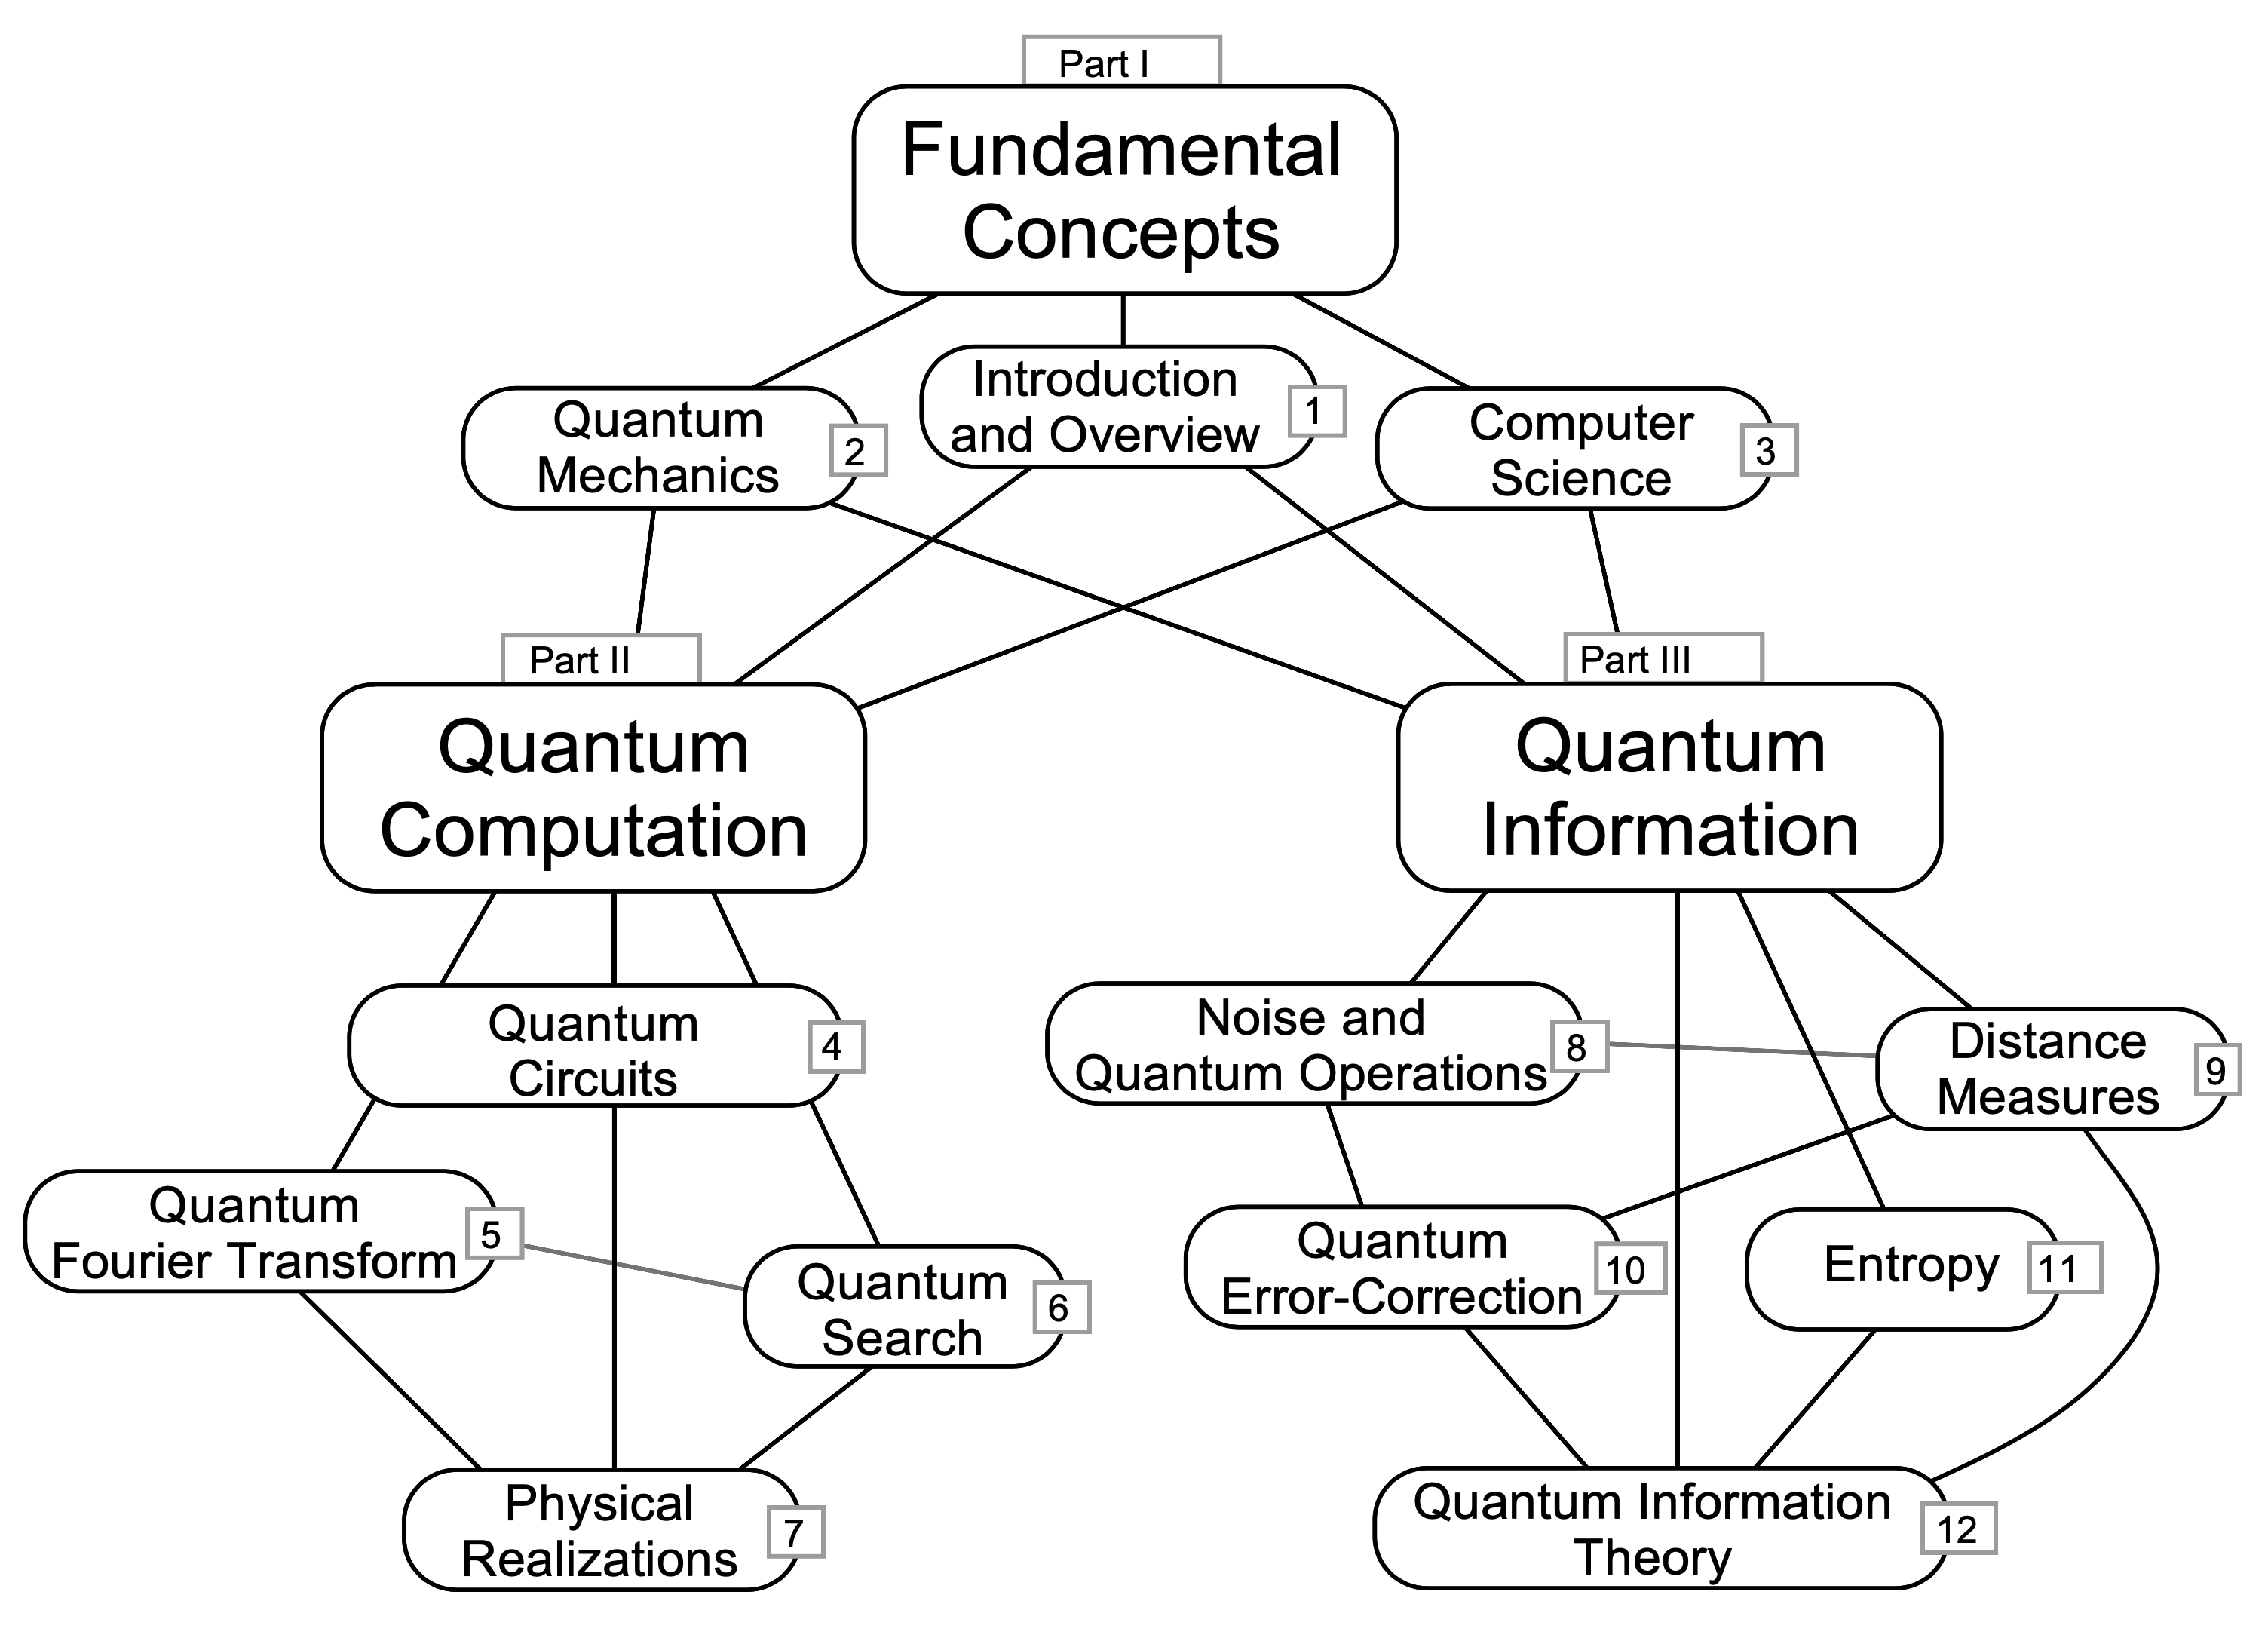
\includegraphics[width=\textwidth]{category.png}
  \caption{A big picture for the quantum computation and 
  quantum information field in Issac Chuang's book. The proposal 
  here focuses more on quantum circuits and quantum fourier transform study. }
\end{figure}

\subsection*{Quantum Gates, Quantum Circuit, and Quantum Computation}
Clasical computer consists of wires and logic gates. Similarly, 
the quantum computer takes quantum version and logic gates and act on 
each qubit. The most famous Pauli Matrices, X are used as NOT gates: 
\begin{equation}
  X = \begin{bmatrix}
    0 & 1 \\ 1 & 0 
  \end{bmatrix},
  Y = \begin{bmatrix}
    0 & -i \\ i & 0 
  \end{bmatrix},
  Z = \begin{bmatrix}
    1 & 0 \\ 0 & -1 
  \end{bmatrix}
\end{equation}
Z gate flips the sign of $\ket{1}$ to give $-\ket{1}$ and 
\textit{Hadamard} gate, 
\begin{equation}
  H =  \frac{1}{\sqrt{2}}\begin{bmatrix}
    1 & 1 \\ 1 & -1
  \end{bmatrix}, S = \begin{bmatrix}
    1 & 0 \\ 0 & i
  \end{bmatrix}, T = \begin{bmatrix}
    1 & 0 \\ 0 & exp(i \pi/4)
  \end{bmatrix}
\end{equation}
Hadamard gate turns $\ket{0}$ into $(\ket{0}+\ket{1})/\sqrt{2}$, and 
$\ket{1}$ into $(\ket{0}-\ket{1})/\sqrt{2}$, phase gate S and $\pi/8$ gate T 
have some algebraic relation with H that $H = (X+Z)/\sqrt{2}$ and 
$S = T^2$. For rotation matrix around X, Y, Z, rotates around x, y, z axes, 
they are defined by equation:
$$R_{\eta}(\theta) = e^{-i \theta \eta /2} = \cos \frac{\theta}{2}I -i \sin \frac{\theta}{2} \eta, \ \ \ \eta \in \{X,Y,Z\}$$
Some important theorem likes Z-Y decomposition for a single qubit 
exits. Suppose U is a unitary operation on a single qubit. Then there exist
real numbers $\alpha, \beta, \gamma, \delta$ such that 
\begin{equation}
  U = e^{i \alpha} R_z(\beta) R_y (\gamma) R_z(\delta)
\end{equation}

\subsubsection*{Controlled Operations}
Here are some controlled openeration with CNOT gate. The core 
idea for controlled operation is "If A is true, then do B". On 
single qubit, in terms of the computational basis, the action
of the CNOT is given by $\ket{c} \ket{t} \rightarrow \ket{c} \ket{t \bigoplus c }$,
which means that the control qubit is set to $\ket{1}$ then the target
qubit is flipped, otherwise the target qubit is left alone. Thus, 
in the computational basis $\ket{control, target}$ the matrix representation
of CNOT is: 
\begin{equation}
  \begin{bmatrix}
    1 & 0 & 0 & 0 \\
    0 & 1 & 0 & 0 \\
    0 & 0 & 0 & 1 \\
    0 & 0 & 1 & 0 
  \end{bmatrix}
\end{equation}
which could also replace by \textit{controlled-U} operation. 
\begin{figure}[h]
  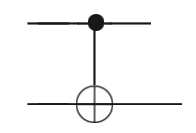
\includegraphics[width=0.20\textwidth]{cnot.png}
  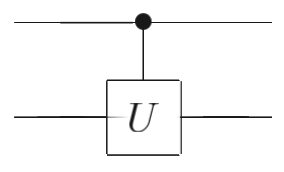
\includegraphics[width=0.24\textwidth]{cnot-u.png}
  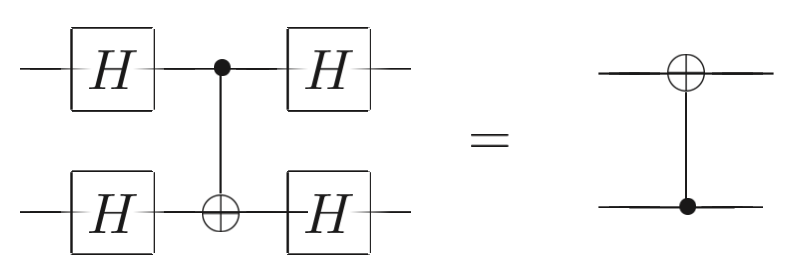
\includegraphics[width=0.48\textwidth]{cnot-h.png}
  \caption{Some circuit representation of control operation}
\end{figure}
\subsection*{Encoding Classical Data into Quantum States}
Quantum Encoding is a process to transform classical information into quantum 
states. In order to use quantum algorithms to solve classical problems, 
such encoding is unavoidable. The simple concept is quantum circuit acts on 
$\ket{0^n}$ state, where n is the number of qubits. Based on different 
requirements, the style of requirement is different. The first three are 
most basic ones and the last two require more depth. 

\subsubsection*{Basis Encoding}
Conceptually the simplest one, encodes an n-bit binary string to an n-qubit 
quantum state $\ket{x} = \ket{i_x}$, where $\ket{i_x}$ is a computational
basis state. Concrete example: $ x =1011 $ maps to $\ket{1011}$

\subsubsection*{Amplitude Encoding}
Vector $x$ of length $N$ into amplitudes of an n-qubit quantum 
state with $n = [log_2(N)]$ and $
  \ket{x} = \sum^N_i x_i \ket{i} $
and $\ket{i}$ is the computational basisi for the Hilbert space. Since 
the classical information forms the amplitudes of a quantum state, the 
input needs to satisfy the normalization condition. For instance, 
$x1 = \begin{bmatrix}
  1/2 \\ 1/2 \\ -1/2 \\-1/2
\end{bmatrix}$, the quantum state will be written as: 
$\ket{x1} = \frac{1}{2} \ket{00} + \frac{1}{2} 
\ket{01} - \frac{1}{2} \ket{10} - \frac{1}{2} \ket{11}$
similarly, for $x2 = \begin{bmatrix}
  1/\sqrt{3} \\ 1/\sqrt{3} \\ -1/\sqrt{3} 
\end{bmatrix}$ the state would be:
$\ket{x2} = \frac{1}{\sqrt{3}} \ket{00} 
+ \frac{1}{\sqrt{3}} \ket{01} - \frac{1}{\sqrt{3}} \ket{10} $

\subsubsection*{Angle Encoding}
Angle encoding uses rotation gates to encode the classical information x. 
The classical information determines angles of rotation gates:
\begin{equation}
  \ket{x} = \bigotimes_i^n R(x_i) \ket{0^n}
\end{equation}
R can be one of the rotation gate $R_x$, $R_y$, and $R_z$. Usually, the 
number of qubits used for enoding is equal to the dimension of vector. For example, 
if $x = \begin{bmatrix}
  \pi \\ \pi \\ \pi 
\end{bmatrix}$, angle encoding rotates every qubit around Y-axis (if we choose $R_y$)
for degree $\pi$, the corresponding quantum state is then $\ket{x} = Ry(\pi) \ket{0} Ry(\pi) \ket{0} Ry(\pi) \ket{0}$
, which indicates the result is $\ket{111}$.

\subsubsection*{IQP Style Encoding}

\subsubsection*{Hamiltonian Evolution Ansatz Encoding}


\subsection*{Quantum Classifier}

\begin{figure}[h]
  \begin{center}
    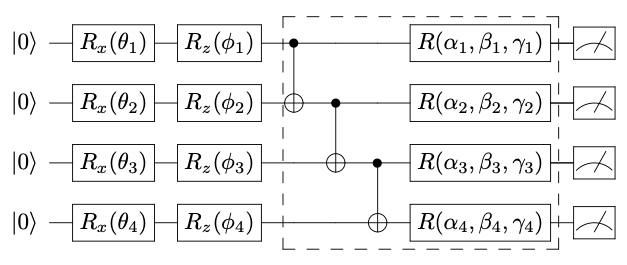
\includegraphics[width=0.58\textwidth]{vqc.png} 
    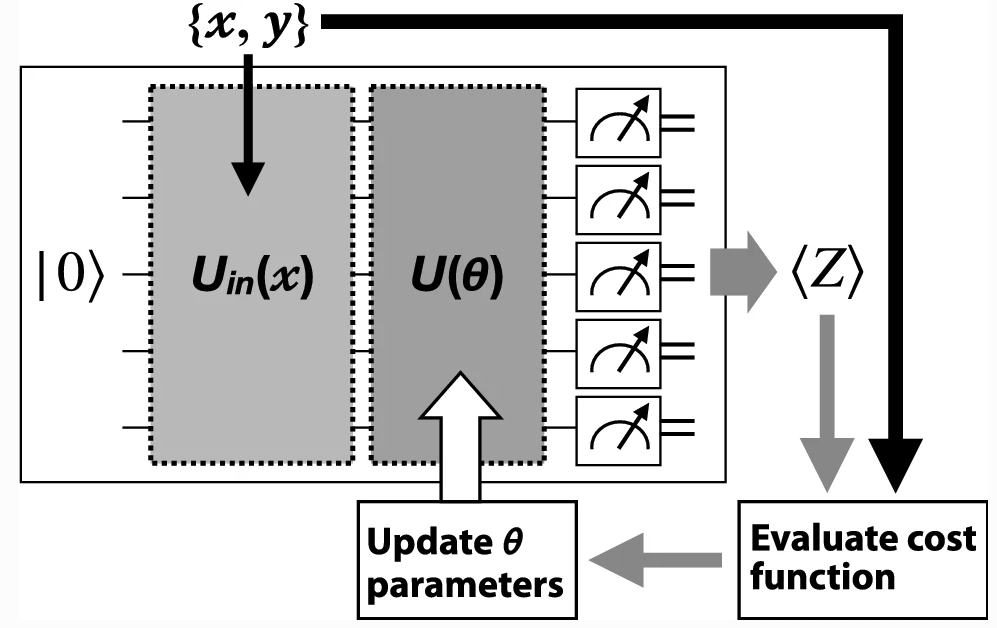
\includegraphics[width=0.38\textwidth]{vqc1.png} 
  \end{center}
  \caption{The generic variational quantum circuit 
  architecture and procedure for optimization. The 
  inputs go through encoding, the unitary matrices, 
  measurement, lost function evalution and then 
  update parameters.}
\end{figure}

The lost function could be the simplest one: 
\begin{equation}
  L (\theta) = \sum^N_{k=1} \frac{1}{N} |\tilde{y}^k - y^k|^2
\end{equation}
\subsection*{Quantum Fourier Transform Phase Estimation}
Suppose a unitary operator U has an eigenvalue $\ket{u}$ with 
eigenvalue $e^{2 \pi i \varphi}$, where the value of 
$\varphi$ is unknown. The goal of the 
phase estimation algorithm is to estimate $\varphi$.
\newline
\textbf{Inputs:} (1) A black box which performs a 
controlled-$U^j$ operation, for integer j. (2) an 
eigenstate $\ket{u}$ of U with eigenvalue $e^{2 \pi i \varphi}$, and 
(3) $t = n + [log(2+\frac{1}{2 \epsilon})]$ qubits initialized 
to $\ket{0}$ \newline
\textbf{Outputs:} An n-bit approximation $\tilde{\varphi_u}$ to $\varphi_u$ \newline
\textbf{Runtime:} $O(t^2)$ operations and one call to controlled-$U^j$
black box. Succeeds with probability at least $1-\epsilon$. \newline
\textbf{Procedure}: 
\begin{enumerate}
  \item $\ket{0}\ket{u}$  initial state
  \item $\rightarrow \frac{1}{\sqrt{2^t}} \sum^{2^t -1}_{j=0} \ket{j}\ket{u} $ create superposition
  \item $\rightarrow \frac{1}{\sqrt{2^t}} \sum^{2^t -1}_{j=0} \ket{j} U^j \ket{u} $ apply black box
  \item $= \frac{1}{\sqrt{2^t}} \sum^{2^t -1}_{j=0}  e^{2 \pi i j \varphi_u} \ket{j} \ket{u} $ result of black box 
  \item $\rightarrow \ket{\tilde{\varphi_u}} \ket{u}$
  \item  $\rightarrow \tilde{\varphi_u}$
\end{enumerate}

\subsection*{Quantum Fourier Transform Shor's Algorithm}

\textbf{References}
\begin{enumerate}
  \item Hamiltonian Evolution Ansatz Encoding: \href{https://journals.aps.org/prb/abstract/10.1103/PhysRevB.102.235122}{Strategies for solving the Fermi-Hubbard model on near-term quantum computers}
\end{enumerate}

\end{document}


% Overall view of the research proposal 
% Interviewer 
% Will your master transfer 
% How to encode 
% There are 

% What will be the things other than encoding?
% How to run the algorithm if Quantum Computer not 
% New idea on signal processing? Doing the translation is 
% bring the novelty part to the front. 
% Avoid doing the implementation 

% Highlight the major contribution of the proposal
% 15minutes Slides: present the main idea 
% giving people some impression. 

% Heat Kernel or Diffusion Kernel. Typical Machine 
% Learning Stuff. 

% Restructure the research proposal: 
% Don't have idea of what quantum machanic is. 
% A single slide for people understand how 
% quantum state: resembles with machine learning. 
% Keep the flow 
% They may have problems with technical issues. 
% How my project will contribute a lot for the 
% field. 
% How we know things? How we know to bring the games 
% into the
% We don't have quantum computer here. 
% How I going to test algorithms: 
% emulation on super computer. more funding. 
% some example: Pixel and image. 

% You can image one in the Linear vector space. 
% explain things in engineering department's view. 
% Audience are different people. 
% Why would you like to come to engineering department? 
% Novel contribution to the signal processing field?
% What are the novel things in Quantum Machine Learning? 
% 

\newpage
\bibliography{references}